\section{Definitions and Problem Statement}
\seclabel{problem}

We consider the problem of finding a of parallel-jaw grasps with maximum probability force closure, $P_F$, on a 3D object model under uncertainty in object pose, gripper pose, and friction coefficient using a database of 3D object models annotated with grasps and the $P_F$ of each.
We assume the object shape is exactly known and provided as a signed distance function (SDF) $f: \mathbb{R}^3 \rightarrow \mathbb{R}$~\cite{mahler2015gp, newcombe2011kinectfusion}, which is zero on the object surface, positive outside the object, and negative inside the object (when the object is watertight). 
We also assume that the object is specified in units of meters and the object center of mass $\bz \in \mathbb{R}^3$ is known.
Furthermore, we assume soft-finger contacts between the gripper and object~\cite{zheng2005} and that the gripper jaws are opened to their maximal width $w \in\bR$ before closing on the object.
%and known uncertainty in object pose, gripper pose relative to the object, and friction coefficient, described in detail in \seclabel{uncertainty} below. 

\subsection{Grasp and Object Parameterization}
\seclabel{grasp-param}
Our grasping parameterization is illustrated in~\figref{grasp-model}.
Let $\bg = (\bx, \bv)^T$ be a parallel-jaw grasp parameterized by the centroid of the jaws in 3D space $\bx \in \mathbb{R}^3$ and an approach direction, or axis, $\bv \in \bS^2$.
Let $f: \mathbb{R}^3 \rightarrow \mathbb{R}$ be a signed distance function (SDF) representing an object's geometry~\cite{mahler2015gp, newcombe2011kinectfusion}.
We denote by $\mS = \{\by \in \bR^3 \big| f(\by) = 0\}$ the surface of an object, and assume that all points are specified with respect to a reference frame centered at the object center of mass $\bz$ and oriented along the principal axes of $\mS$.
Let $\mG = \{ [(\bx, \bw) \big| \bx \in \mathbb{R}^3, \bv \in \bS^2\}$ denote the space of all grasps and $\mH = \{ \mO = \{\bz, f(\cdot)\} \big|  \bz \in \mathbb{R}^3, f \in \mF\}$ denote the space of all objects, where the $\mF$ is the space of all SDFs for closed and compact surfaces.
We denote by $\mM = \mG \times \mH$ the joint space of all parallel-jaw grasps and objects, also known as a Grasp Moduli Space~\cite{pokorny2013grasp}.

\begin{figure}[t!]
\centering
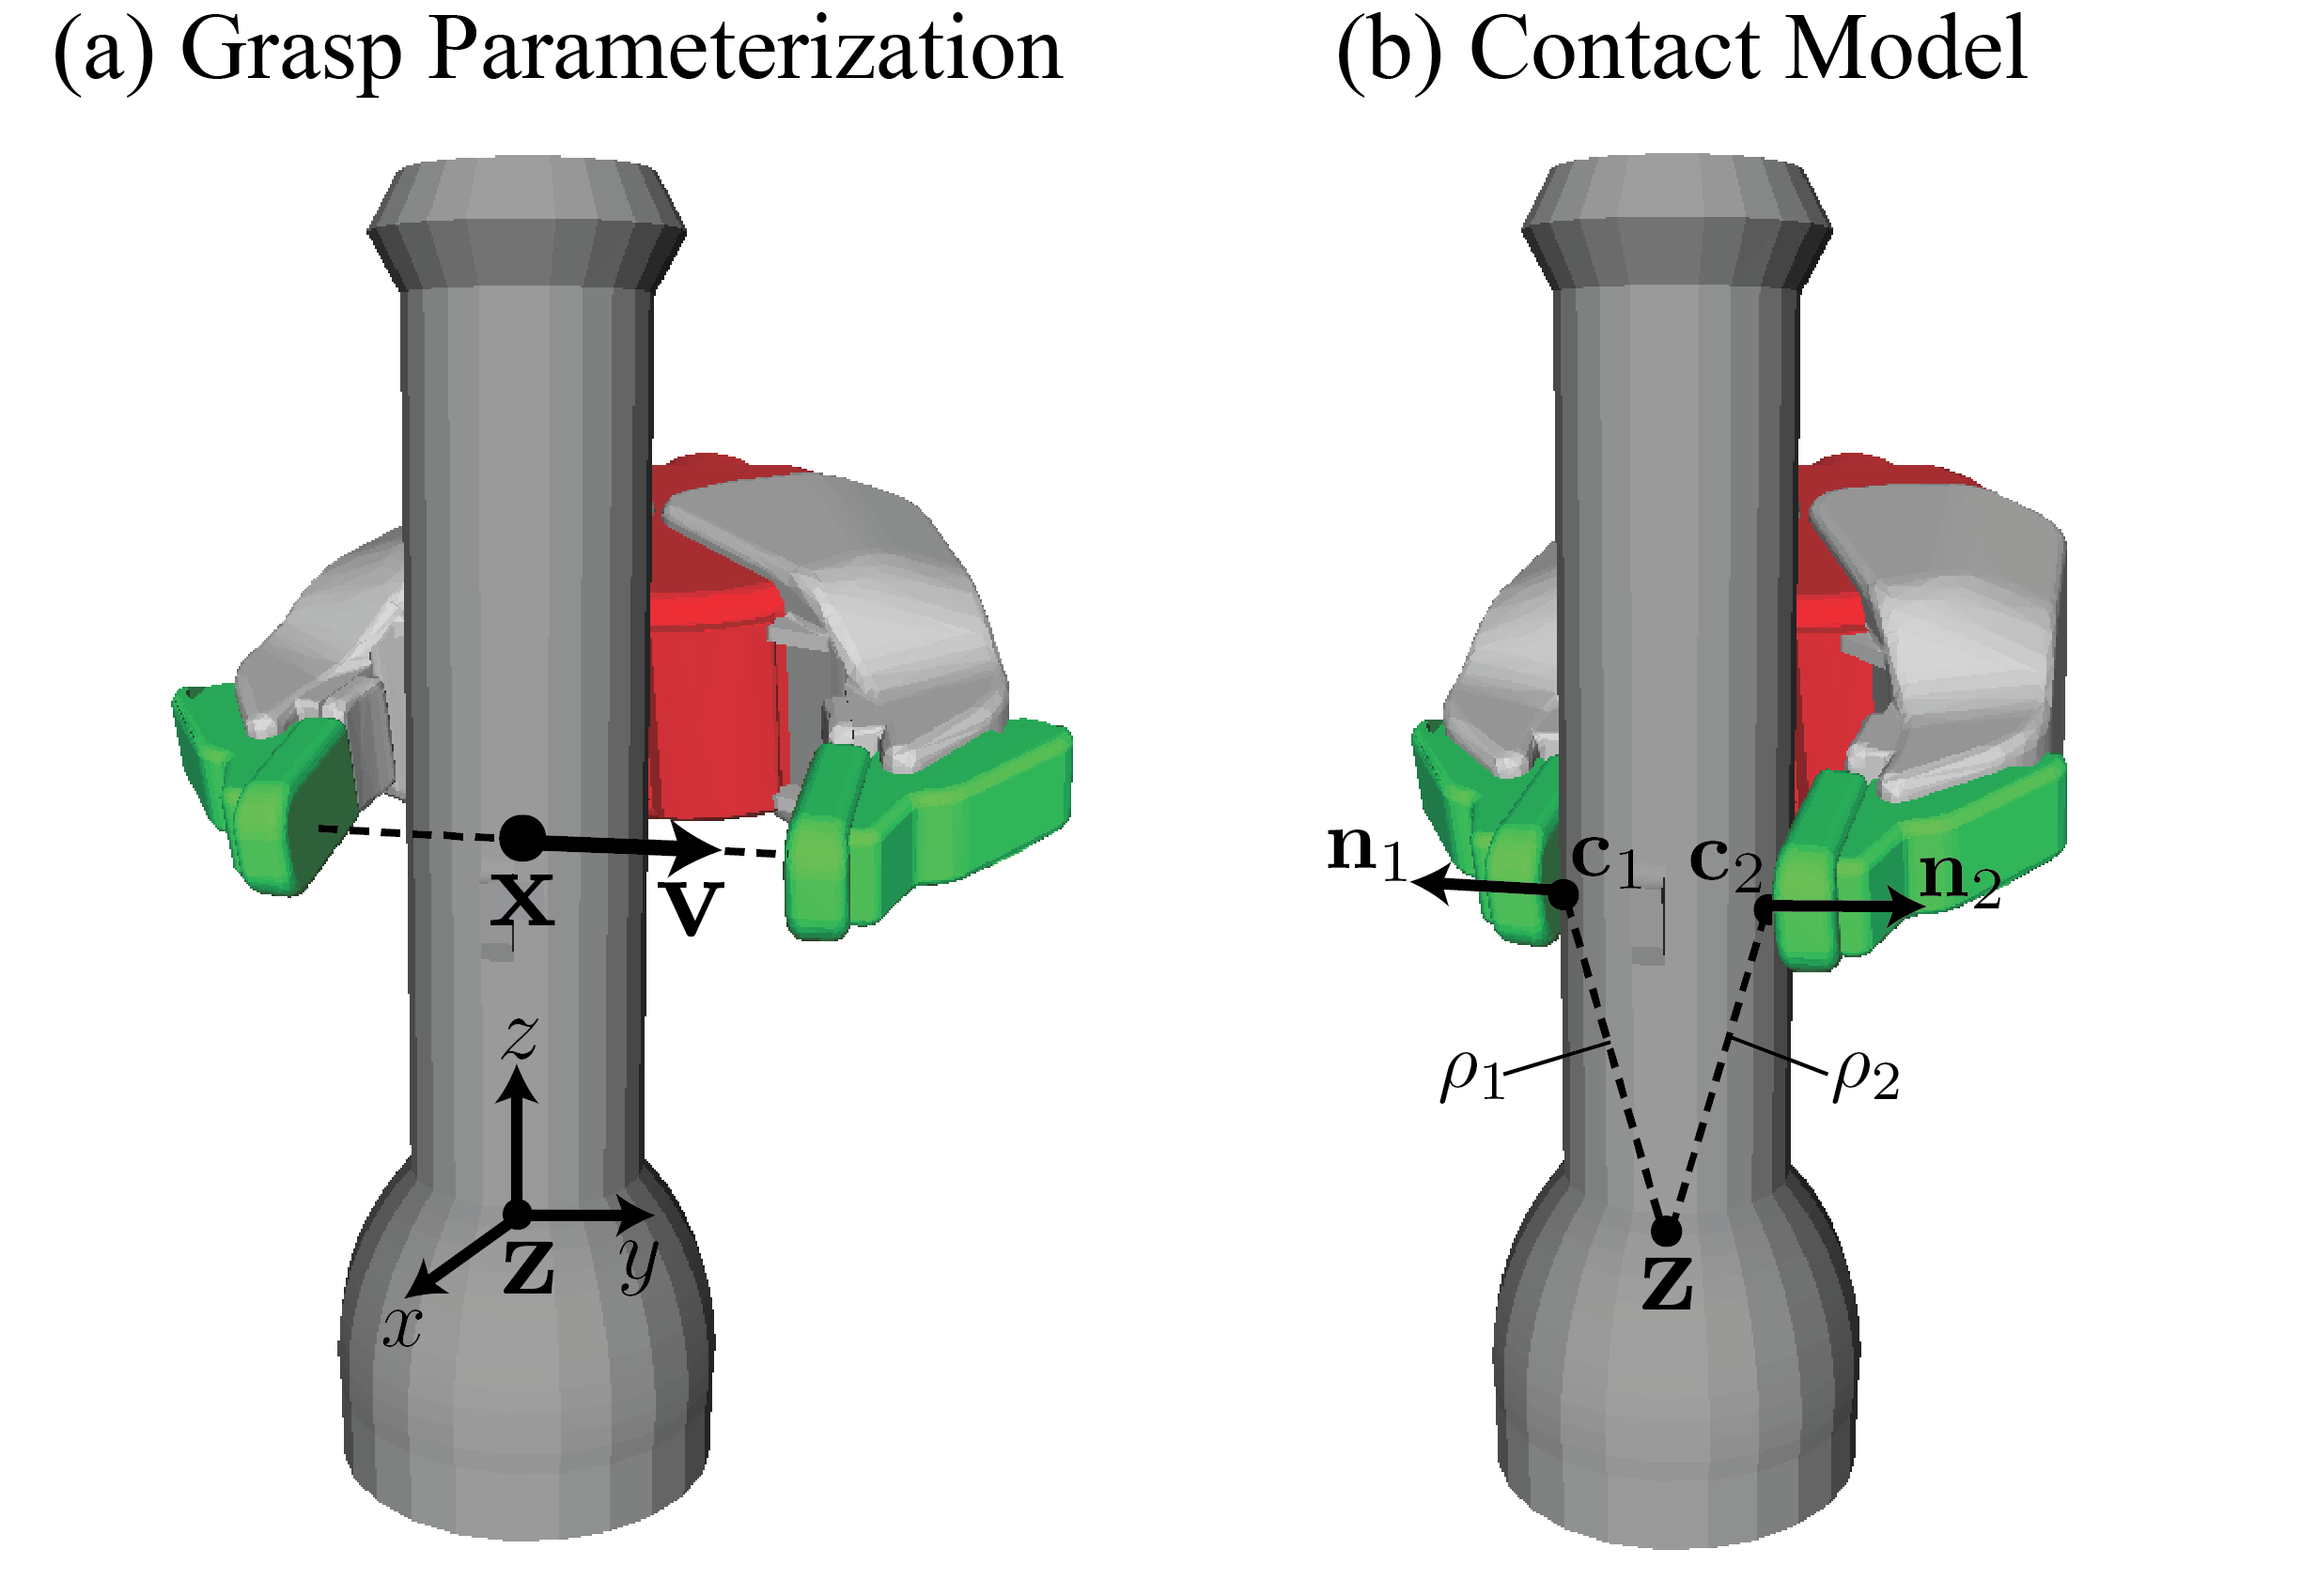
\includegraphics[scale=0.4]{figures/illustrations/dexnet_grasping_model.png}
\caption{Illustration of our grasp parameterization and contact model. (Left) We parameterize parallel-jaw grasps by the centroid of the jaws $\bx \in \mathbb{R}^3$ and approach direction, or direction along which the jaws close, $\bv \in \bS^2$. The grasp parameters $\bx$ and $\bv$ are specified with respect to a coordinate frame located at the object center of mass $\bz$ and oriented along the principal directions of the object. (Right) The jaws are closed until contacting the object surface at locations $\bc_1, \bc_2 \in \mathbb{R}^3$, at which the surface has normals $\bn_1, \bn_2 \in \bS^2$. The contacts are used to compute the moment arms $\rho_1 = \bc_1 - \bz$ and $\rho_2  = \bc_2 - \bz$. From these parameters we can derive the forces and torques that the gripper can apply to the object. }
\figlabel{grasp-model}
\vspace*{-15pt}
\end{figure}

\subsection{Sources of Uncertainty}
\seclabel{uncertainty}
We assume Gaussian distribuions on 3D object pose, gripper pose, and friction coefficient resulting from sensing uncertainties and missing data extended from the 2D model of Laskey et al.~\cite{laskey2015bandits}.
Let $\upsilon \sim \mN\left(\mathbf{0}, \Sigma_{\upsilon}\right)$ denote a zero-mean Gaussian on $\bR^6$ and $\mu_{\xi} \in SE(3)$ be a mean object pose.
Following the model of Barfoot and Furgale~\cite{barfoot2014associating}, we define the object pose random variable $\xi = \exp\left( \upsilon^{\wedge} \right) \mu_{\xi}$, where the $\wedge$ operator maps from $\bR^6$ to the Lie algebra $\mathfrak{se}(3)$.
Let $\nu \sim \mN\left(\mu_{\nu}, \Sigma_{\nu}\right)$ denote a Gaussian distribution on gripper pose with mean $\mu_{\nu} \in \mG$.
Let $\gamma \sim \mN\left(\mu_{\gamma}, \Sigma_{\gamma} \right)$ denote a Gaussian distribution on friction coefficient with mean $\mu_{\gamma} \in \mathbb{R}$.
We denote by $\hat{\xi}, \hat{\nu},$ and $\hat{gamma}$ samples of object pose, gripper pose, and friction, respectively. 
%Theses sources of uncertainty might be estimated based on prior models of repeatability in gripper actuation or from the posterior variance in object pose or friction coefficient in estimates based on sensor data.

\subsection{Contact Model}
\seclabel{contact}
Our contact model is illustrated in the right panel of \figref{grasp-model}.
Given a grasp $\bg$ with width $w$ on an object $\mO$ and samples of object pose, gripper pose, and friction, let $\bc_i \in \mathbb{R}^3$ for $i \in {1, 2}$ denote the 3D contact location between the $i$-th gripper jaw and surface.
Each contact $\bc_i = \bx + s_i (t_i^* - w / 2) \bv$ where
\begin{align*}
	t_i^* &= \minimum{t \geq 0} t \text{ such that } f\left(\bx + s_i (t - w / 2) \bv\right) = 0,
\end{align*}
\noindent$s_1 = -1$, and $s_2 = 1$~\cite{mahler2015gp}.

Given contact points, let $\bn_i = \nabla f(\bc_i) / \| \nabla f(\bc_i) \|_2$ denote the surface normal at contact $\bc_i$ with tanget vectors $\bt_{i,1}, \bt_{i,2} \in \bS^2$.
To compute the forces that each contact can apply to the object for a sampled friction coefficient $\hat{\gamma}$, we discretize the friction cone at contact $i$~\cite{pokorny2013classical} into a discrete set of $l$ facets with vertices $\mF_{i} = \left\{ \bbf_{i,j} = \bn_i + \hat{\gamma} \cos \left( \frac{2 \pi j}{l} \right) \bt_{i,1} + \hat{\gamma} \sin \left( \frac{2 \pi j}{l} \right) \bt_{i,2} \text{ for } j = 1, ..., l \right\}$.
Each force $\bbf_{i,j}$ can exert a corresponding torque $\tau_{i,j} = \bbf_{i,j} \times \rho_i$ where $\rho_i = (\bc_i - \bz)$ is the moment arm at contact $i$.
Under our soft contact model, each contact $\bc_i$ exerts an additional wrench $\bw_{i,l+1} = (\mathbf{0}, \bn_i)$~\cite{zheng2005}.
Thus the set of all wrenches that can be applied by a grasp $\bg$ under our model is $\mW = \{ \bw_{i,j} = (\bbf_{i,j}, \tau_{i,j}) \big| i = 1, 2 \text{ and } j = 1, ..., l+1\}$.

\subsection{Quality Metric}
\seclabel{quality}
In this work we use the probability of force closure, or the ability to resist external force and torques in arbitrary directions~\cite{ferrari1992}, as our grasp success metric.
While we acknowledge that deterministic force closure has not always been reported as a predictor of physical grasp success~\cite{balasubramanian2012physical, diankov2010automated}, we use the probability of force closure because of it has shown promise in physical experiments~\cite{kim2012physically, weisz2012pose} and is relatively inexpensive to evaluate, allowing us to better study the effects of large amounts of data.

Let $F \in \{0, 1\}$ denote the occurence of force closure.
To compute force closure for a grasp $\bg \in \mG$ on object $\mO \in \mH$ given samples of object pose $\hat{\xi}$, gripper pose $\hat{\nu}$, and friction coefficient $\hat{\gamma}$, we first compute the set of possible contact wrenches $\mW$.
Then $F = 1$ if the origin lies within the convex hull of the contact wrench set, $\mathbf{0} \in Conv(\mW)$~\cite{weisz2012pose}.

\subsection{Objective}
The probability of force closure for a grasp $\bg$ on object $\mO$ is $P_F(\bg, \mO) = \mathbb{P}\left(F = 1 \mid \bg, \mO, \xi, \nu, \gamma \right)$.
We are interested in finding $\bg^*$,the grasp that maximizes the probability of force closure $P_F(g)$~\cite{kim2012physically, laskey2015bandits, mahler2015gp, weisz2012pose} over a budgeted maximum number of samples $T$.
To perform this as quickly as possible we maximize over the sum of the $P_F$ for all sampled grasps~\cite{laskey2015bandits, srinivas10gaussian}:

\vspace{-2ex}
\begin{align}
	\underset{g_{I(1)}, ..., g_{I(T)} \in \mG}{\text{maximize }} \sum \limits_{t=1}^T P_F(g_{I(t)}). \label{eq:objective}
\end{align}
\noindent where $I(i)$ denotes the grasp selected at time $t$.

As the maximization over the continuous space $\mG$ is computationally expensive, past work has solved this objective by evaluating a discrete set of $K$ candidate grasps $\Gamma = \left\{ \bg_1, ..., \bg_K \right\}$ with Monte-Carlo integration~\cite{kehoe2012toward, weisz2012pose} or Multi-Armed Bandits(MAB) ~\cite{laskey2015bandits}.
In this work, we extend the MAB model of~\cite{laskey2015bandits} to 3D and to leverage similarities between grasps and prior objects in Dex-Net to reduce the samples needed to converge to $\bg^*$.